\documentclass[12pt, journal, onecolumn]{IEEEtran}
\raggedbottom
%
\usepackage{instructivo}  % Commands for multiple choice
\graphicspath{{./}{./fig/}}

\usepackage[natbib=true,style=trad-unsrt,backend=biber]{biblatex}

\addbibresource{literatura.bib}
\usepackage{multirow}
\usepackage{graphicx}
\usepackage{array}
\usepackage{float}
\usepackage{capt-of}
\newcolumntype{C}{>{\centering\arraybackslash}X}
% correct bad hyphenation here
\hyphenation{op-tical net-works semi-conduc-tor}


\begin{document}
	%
	% paper title
	% Titles are generally capitalized except for words such as a, an, and, as,
	% at, but, by, for, in, nor, of, on, or, the, to and up, which are usually
	% not capitalized unless they are the first or last word of the title.
	% Linebreaks \\ can be used within to get better formatting as desired.
	% Do not put math or special symbols in the title.
\title{Proyecto: Semáforo Vehicular y Peatonal}
	
	
\author{Gerald~David~Blanco-Sáenz,~\IEEEmembership{Estudiante,~ITCR},~Melanie~Espinoza-Hernandez,~\IEEEmembership{Estudiante,~ITCR},~Nayshell~Freckleton-White,~\IEEEmembership{Estudiante,~ITCR} 
	y~Pablo~Cabrera-Montealegre,~\IEEEmembership{Estudiante,~ITCR}}
	
	
	% The paper headers
\markboth{EL3215 Laboratorio de Electrónica Analógica, IS2026}%
{EL3215 Laboratorio de Electrónica Analógica}
	
	
	% make the title area
\maketitle
	
\begin{abstract}
		Se propone el diseño de un sistema de semáforo vehicular y peatonal, cuyo objetivo principal es simular un cruce vehicular completo mediante la gestión del flujo de tránsito y la interacción a través de solicitudes peatonales. El sistema incorpora señalización visual (rojo, amarillo, verde) y auditiva, control de tiempos regresivos mediante displays, y una etapa de conversión de energía de corriente alterna (CA) a corriente directa (CD). En este primer avance, se documenta exclusivamente la etapa de alimentación del circuito, la cual es responsable de proveer los niveles de tensión regulados adecuados para el funcionamiento de las etapas analógicas y digitales posteriores.
\end{abstract}
	
\section{Introducción}
	Los sistemas de control de tráfico son fundamentales para la regulación segura y eficiente de la movilidad vehicular y peatonal en entornos urbanos. Estos sistemas integran elementos de temporización, señalización visual y auditiva, así como mecanismos de interacción con los usuarios. En el contexto de la ingeniería electrónica, el diseño de un sistema de semáforo permite aplicar conceptos relacionados con la generación de señales, temporización, control lógico, visualización de información y procesamiento de señales de audio. Además, representa un ejemplo claro de integración de subsistemas analógicos y digitales en una aplicación real. 
	
	Este proyecto se enfoca en el diseño e implementación de un sistema completo de semáforo vehicular y peatonal, utilizando componentes electrónicos discretos y circuitos digitales básicos, evitando el uso de dispositivos programables de acuerdo con las especificaciones. El objetivo principal de este primer documento es presentar la propuesta de diseño de cada etapa del sistema, detallando sus componentes y la justificación de las decisiones de diseño.
	
	\section{Objetivos}
	\subsection{Objetivo General}
	Introducir al estudiante ante un problema de ingeniería en donde requiera poner en práctica las habilidades y conceptos adquiridos en el uso de las herramientas de simulación, equipos de medición, prototipado y ensamble de circuitos eléctricos transistorizados por medio de circuitos impresos.
	
	\subsection{Objetivos Específicos}
	\begin{itemize}
		\item Introducir al estudiante en el diseño de ingeniería bajo el establecimiento de una solución a un problema planteado.
		\item Utilizar herramientas de simulación en la etapa de diseño de sistemas electrónicos que integren etapas analógicas y digitales.
		\item Desarrollar habilidades de implementación de sistemas electrónicos bajo el apoyo de equipo especializado para mediciones.
		\item Adquirir conocimiento y habilidades necesarias para el diseño e implementación de circuitos impresos o PCB para ensamble de circuitos eléctricos.
		\item Fomentar las habilidades requeridas para el trabajo en equipo en proyectos de ingeniería.
	\end{itemize}
	
	\section{Alimentación}
	\subsection{Descripción}
	Para el funcionamiento del semáforo eléctrico y sus respectivos sistemas lógicos, se requiere una fuente de alimentación que convierta la energía proveniente de la red eléctrica de 120\,$\text{V}_{\text{rms}}$ a 60\,Hz en niveles de tensión de corriente directa (CD) regulados y ajustados. Estos voltajes son vitales para cumplir con las condiciones de operación de las compuertas lógicas, los circuitos de temporización y las etapas de potencia para la señalización visual y acústica.
	
	El circuito convertidor de CA a CD incluye los siguientes componentes principales: un transformador reductor, un puente rectificador de onda completa, capacitores de filtrado y reguladores de voltaje lineal. Estos elementos actúan en conjunto para entregar las tensiones estables que requiere el resto del sistema, protegiendo los componentes de variaciones indeseadas.
	
	\subsection{Diagrama del circuito}
	% Descomente y ajuste el nombre de la imagen:
	\begin{figure}[h]
		\centering
		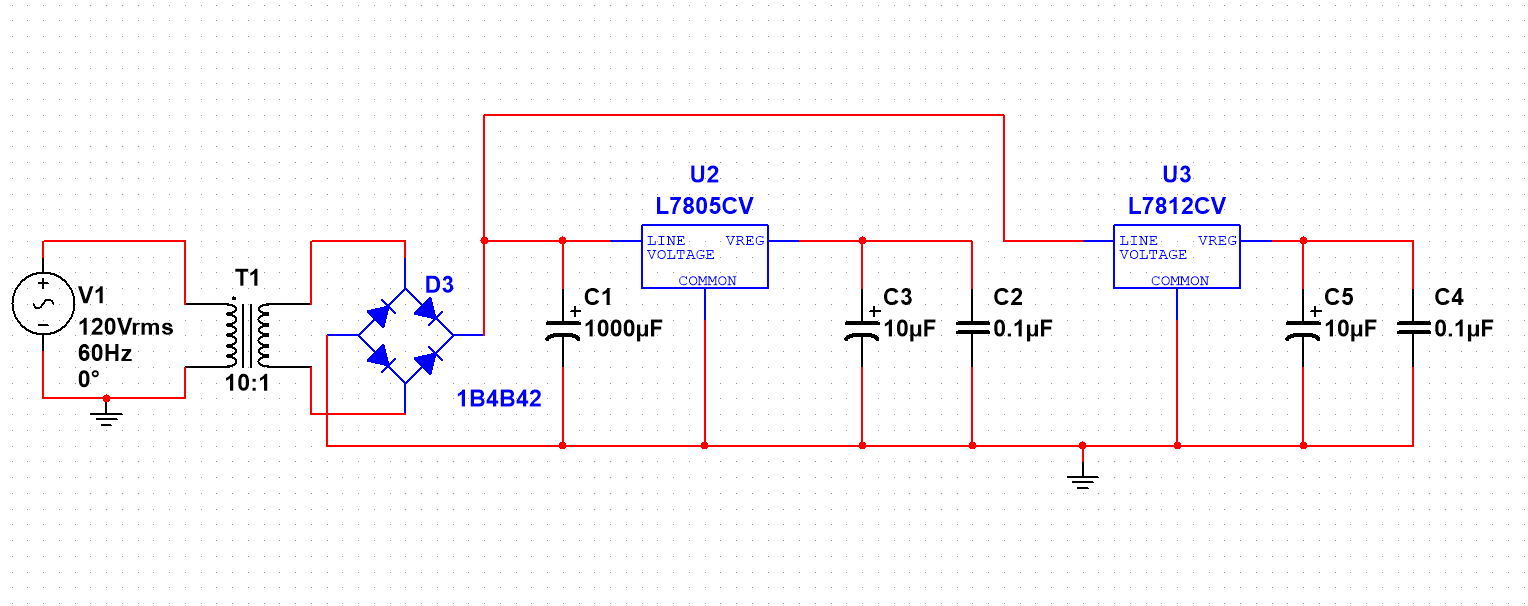
\includegraphics[width=0.8\textwidth]{diagrama_alimentacion.png}
		\caption{Diagrama del circuito de Alimentación.}
		\label{fig:alimentacion}
	\end{figure}
	
	\subsection{Justificación de diseño}
	El diseño del circuito de alimentación de la Fig. \ref{fig:alimentacion} se fundamenta en la necesidad de convertir los 120\,$\text{V}_{\text{rms}}$ de corriente alterna (CA) a voltajes de corriente directa (CD) regulados estables, habitualmente de 5\,V para los componentes de lógica digital (TTL/CMOS), y otros voltajes mayores (como 12\,V) si así lo requieren la amplificación de la señal acústica o los arreglos de LEDs de alta luminosidad.
	
	Inicialmente, el transformador reductor disminuye el voltaje de entrada a un nivel seguro y apto para su manipulación. Luego, el puente rectificador de diodos convierte la señal alterna en una señal pulsante en una sola dirección. Para disminuir el rizado de esta señal, se incorporan capacitores de gran valor en capacitancia que filtran las oscilaciones y otorgan una primera etapa de estabilización a la señal.
	
	Finalmente, los reguladores de voltaje integrados (como los de la familia 78XX) proporcionan una salida continua y fija, absorbiendo las variaciones en el consumo de corriente al encender diferentes estados del semáforo. Se agregan capacitores de desacople adicionales en los terminales de entrada y salida de estos reguladores para estabilizar la respuesta transitoria del dispositivo y atenuar posibles ruidos de alta frecuencia introducidos por la conmutación lógica, garantizando así un desempeño ininterrumpido en todo el circuito de control de tráfico.
	
\section{Máquina de estado}
\subsection{Descripción}
Esta subsección describe la parte del circuito que se encarga de controlar la secuencia de iluminación del semáforo, determinando cuál luz se activa, su color y la duración de cada estado. El sketch inicial del circuito se muestra en la Figura \ref{fsm1}. El circuito requiere una tensión de alimentación de 5 $V$, proporcionada por el circuito de alimentación. Para el mejor entendimiento del lector, se va a dividir la máquina en tres bloques funcionales: El generador de reloj (CLK), la máquina de estados principal y la interconexión entre ambos mencionados anteriormente. El diagrama de como construirlo se puede apreciar en la Figura \ref{fsm}.

Para el generador de reloj se implementa un LM555 TIMER configurado para que opere en un modo astable, para ello su pin de $VCC$ va conectado al voltaje de 5 $V$. Para ello se utilizan dos resistencias de $R_1$ =10.5 $k \Omega$ y de $R_2$ = 9.5 $k \Omega$, y dos capacitores de $C_1$ = 10 $\mu F$ y $C_2$ = 0.01 $\mu F$.  $R_1$ se conecta entre la alimentación y al pin de Discharge (pin 7). $R_2$ se conecta entre pin del Discharge y el nodo común de los pines Threshold (pin 6) y el Trigger (pin 2), donde también se conecta $C_1$. $C_2$ se conecta entre el pin Control Voltage (pin 5). $C_1$, $C_2$ y LM555 se conectan al GND.

La máquina de estados principal se compone de una CD4017B, que se encarga de cambiar de estado/salida cada flanco de reloj positivo. La salida del 4017 se decodifica mediante compuertas 74LS32 (OR) para activar los LEDs correspondientes de cada estado, una alimentación de 5 $V$ y tres resistencias de 330 $\Omega$.

La interconexión se compone de 2 compuertas lógicas, una 74LS00 (NAND) y una 74LS32 (OR). Las entradas de la NAND van conectadas a la salida Q0 de la 4017 y su salida va conectada al Reset (pin 4) de la 555. La primera entrada de la OR va conectada al botón peatonal, la segunda va al Output (pin 3) del 555  y su salida va conectada al clk (pin 14) de la 4017. 

\subsection{Diagrama del circuito}
	% Descomente y ajuste el nombre de la imagen:
	
	\begin{figure}[h]
		\centering
		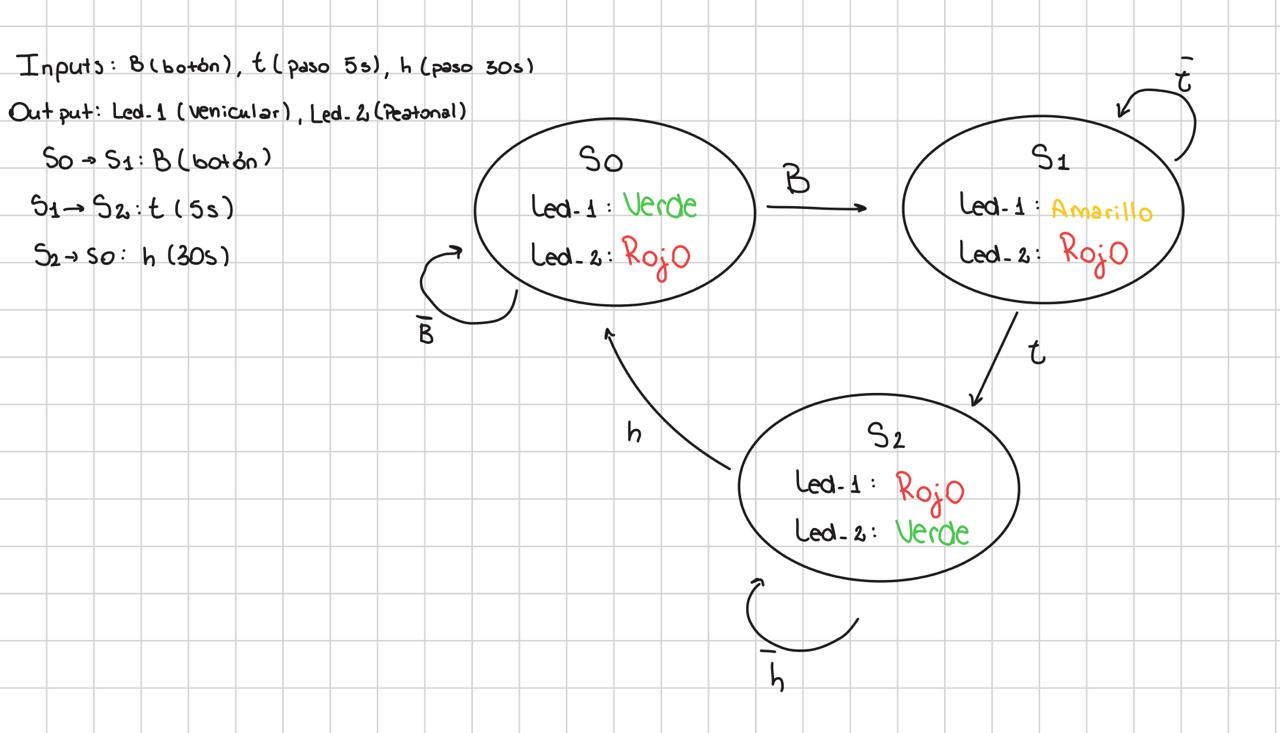
\includegraphics[width=0.7\textwidth]{fsm.jpg}
		\caption{Diagrama inicial del flujo de la máquina de estado.}
		\label{fsm1}
	\end{figure}
	
	\begin{figure}[h]
		\centering
		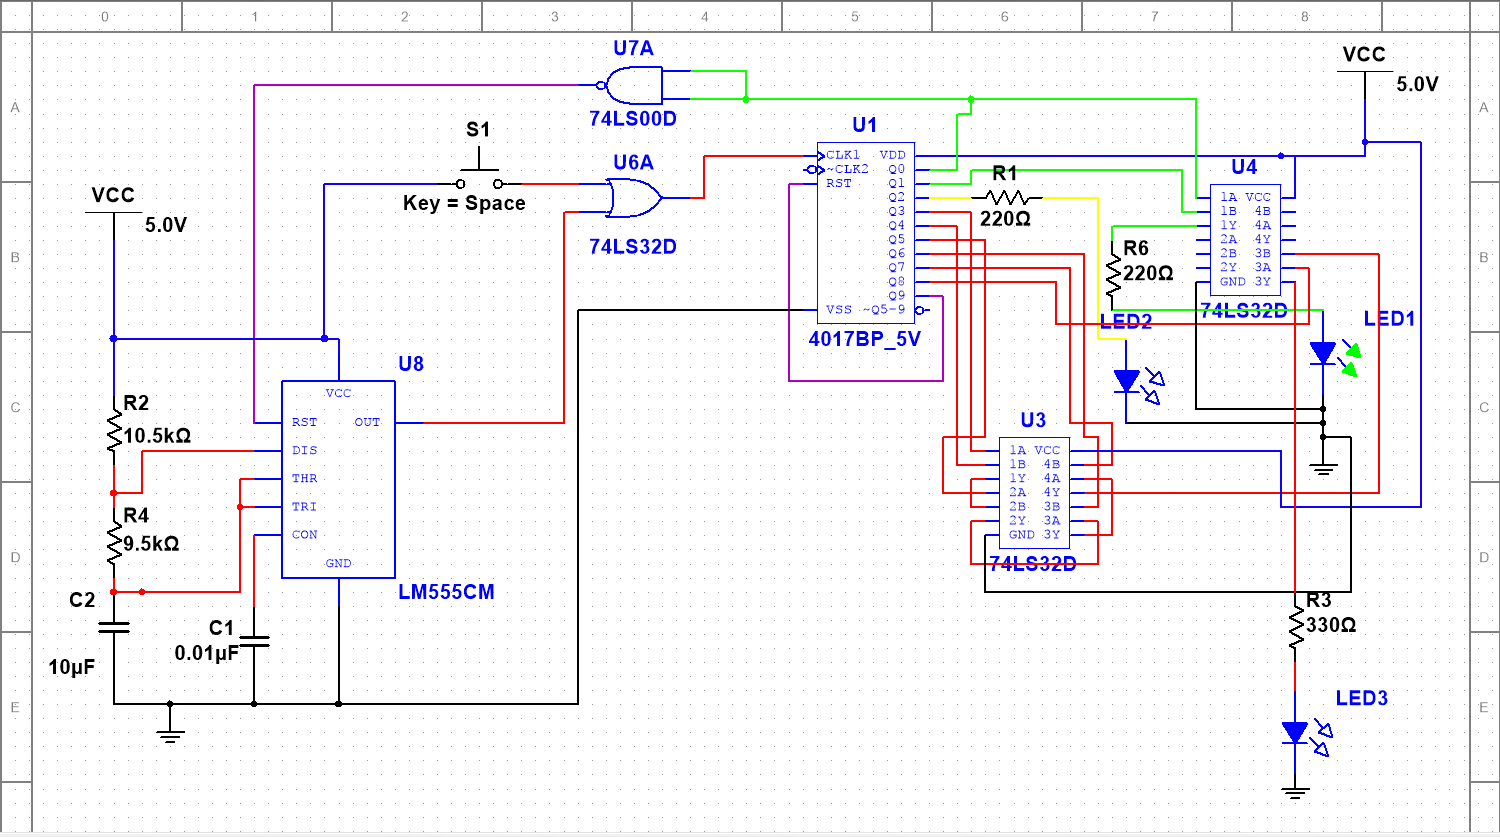
\includegraphics[width=0.9\textwidth]{diagrama_fsm.png}
		\caption{Diagrama del circuito la máquina de estado.}
		\label{fsm}
	\end{figure}
	
	
\subsection{Justificación de diseño}
\subsubsection{Generador de reloj}
El generador de reloj se implementó con el LM555CM en modo astable 
porque este produce una onda cuadrada estable de 5 o 0 $V$ en su salida, lo que es compatible con los niveles lógicos del CD4017. Se llegó a los valores de las resistencias mediante prueba y error. El capacitor $C_2$ se conecta entre el pin Control Voltage (pin 5) y GND con el propósito de filtrar ruido en la tensión de referencia interna del LM555, garantizando una oscilación lo más estable posible.


\subsubsection{Máquina de estado principal}
El CD4017 es un contador de década que activa secuencialmente sus 10 salidas, $Q_0$ a $Q_9$, en cada flanco positivo de reloj. La asignación de salidas se justifica de la siguiente manera:

$Q_0$ corresponde al estado base $S_0$, en el cual el semáforo vehicular permanece en verde indefinidamente hasta que el usuario presione el botón peatonal. En este estado, la lógica de interconexión mantiene el LM555CM detenido, por lo que el contador no avanza ya que esta apagado.
$Q_1$ no tiene ningún LED conectado directamente. Durante las pruebas se determinó que conectar un LED a esta salida causaba que el estado durara un tiempo considerablemente menor al esperado, produciendo un parpadeo que era casi imperceptible. Por esta razón, $Q_1$ se conecta únicamente a una compuerta OR como señal auxiliar para que haya una LED conectada, y el LED amarillo se desplazó a $Q_2$.
$Q_2$ corresponde al estado $S_1$, donde se activa el LED amarillo del semáforo vehicular. Este estado dura exactamente un período de reloj, es decir, aproximadamente 5 $s$.
De $Q_3$ a $Q_8$ se le atribuye al estado $S_2$, donde se activa el LED rojo del semáforo vehicular, durante 30 $s$. Al agrupar 6 salidas consecutivas, el sistema permanece en rojo durante $6 \times 5~\text{s} = 30~\text{s}$, cumpliendo con la especificación de diseño.
Finalmente, $Q_9$ se conecta al pin Reset (RST) del CD4017, forzando el reinicio del contador a $Q_0$ y reiniciando el ciclo completo hasta que el botón peatonal sea presionado nuevamente.

\subsubsection{Interconexión}
La lógica de interconexión cumple dos funciones principales: controlar cuando debe de empezar a funcionar el LM555CM y permitir que el botón peatonal fuerce la transición desde $S_0$ a $S_1$.
La compuerta NAND se usa como una NOT por la necesidad de detener el oscilador cuando el sistema se encuentra en $S_0$. Dado que $Q_0 = 1$ en dicho estado, se invierte esta señal para obtener un nivel bajo en el pin Reset (pin 4) del LM555CM, deteniendo la oscilación. Cuando el contador avanza a cualquier otro estado, $Q_0 = 0$, la salida del inversor pasa a nivel alto y el LM555CM comienza a oscilar libremente, avanzando entre los estados/salidas de manera automática.

La compuerta OR se utiliza ya que se necesita combinar dos fuentes de reloj: el botón peatonal y la salida del LM555CM. En $S_0$, como el 555 está detenido, únicamente el botón puede generar el flanco positivo necesario para hacer que el CD4017BP avance hacia $Q_1$. En los estados siguientes, el botón no interviene y es el LM555CM quien genera los flancos de reloj automáticamente.

\subsection{Gráficas}

\begin{figure}[H]
    \centering
    \begin{minipage}{0.45\textwidth}
        \centering
        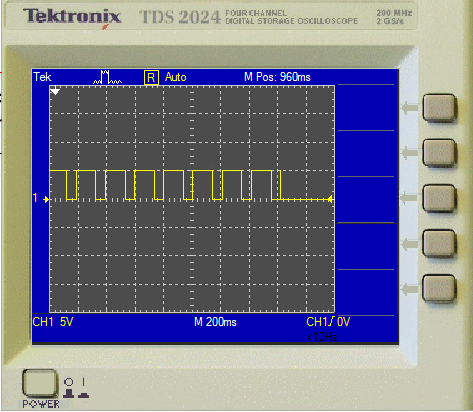
\includegraphics[width=0.9\textwidth]{f0.png}
		\caption{Gráfica de CLK.}
    \end{minipage}
    \hfill
    \begin{minipage}{0.45\textwidth}
        \centering
        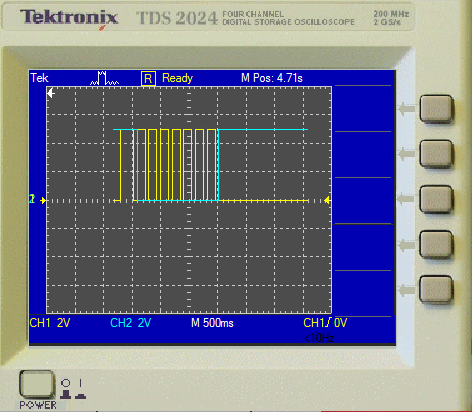
\includegraphics[width=0.9\textwidth]{f1.png}
		\caption{Gráfica de CLK vs $S_0$.}
    \end{minipage}

    \vspace{0.5cm}

    \begin{minipage}{0.45\textwidth}
        \centering
        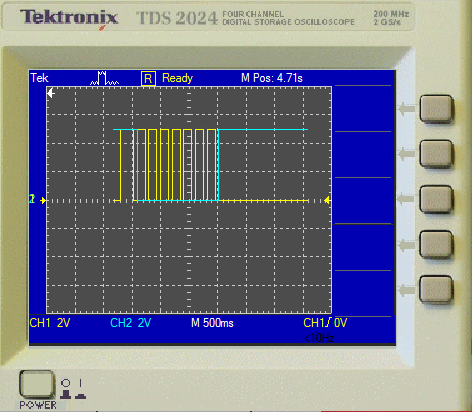
\includegraphics[width=0.9\textwidth]{f1.png}
		\caption{Gráfica de CLK vs $S_0$.}
    \end{minipage}
    \hfill
    \begin{minipage}{0.45\textwidth}
        \centering
        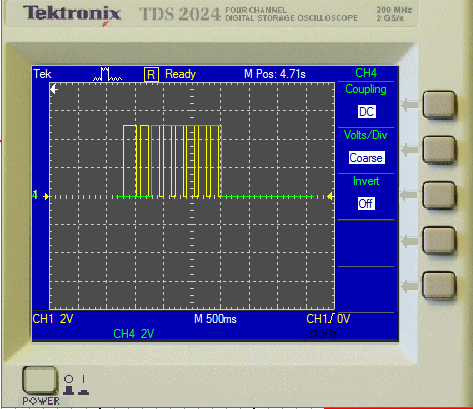
\includegraphics[width=0.9\textwidth]{f3.png}
		\caption{Gráfica de CLK vs $S_2$.}
    \end{minipage}
    \hfill
    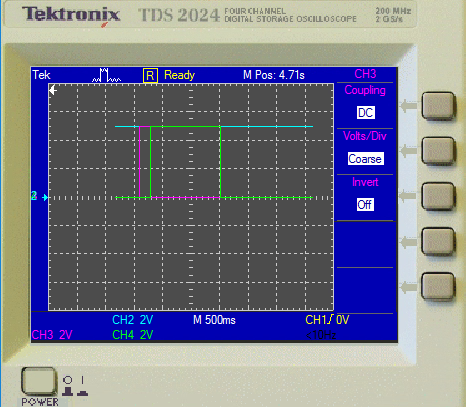
\includegraphics[width=0.4\textwidth]{ftot.png}
	\caption{Gráfica de $S_0$ vs $S_1$ vs $S_2$.}
\end{figure}

\section{Sistema de Señalización Auditiva}

\subsection{Descripción}
Este sistema fue diseñado con el propósito de generar una señal auditiva para los peatones cuando este permitido cruzar la calle. Consiste en generar un sonido periódico cuando el semáforo peatonal se encuentre en verde y que este mismo se acelera una vez que falten cinco segundos para que se vuelva a poner en rojo. 
Tomando en cuenta las especificaciones solicitadas cumpliendo únicamente con el uso de electrónica básica y sin ningún tipo de microcontroladores, se llego a la conclusión que la mejor forma de manejarlo era por medio de osciladores RC con la que se pueden ajustar la frecuencias y compuertas Schmitt Trigger acompañadas de un amplificador para el sonido de salida.
Dado estos requerimientos se pude decir que el sistema completo se divide en cuatro bloques funcionales principales:
\begin{enumerate}
    \item Generación del tono audible.
    \item Generación de la frecuencia de repetición lenta.
    \item Generación de la frecuencia de repetición rápida.
    \item Etapa de selección y amplificación de potencia.
\end{enumerate}
En cuanto al funcionamiento del circuito, todo empieza generando una señal de una frecuencia audible (en este caso unos 2kHz aproximadamente) por medio de un oscilador principal. Se selecciona esta frecuencia ya que se encuentra dentro del rango perceptible por el oído humano siendo perceptible fácilmente.
Adicional a esto, se generan además dos osciladores mas de aproximadamente 1Hz y 5Hz sujetos a modificaciones según las pruebas del circuito ensamblado en físico. Estas señales no funcionan como audio directamente, sino que al combinarse lógicamente generan periodos de activación de la señal de tono según la velocidad que sea deseada y dependiendo directamente del estado del semáforo peatonal.
Dependiendo del estado en el que se encuentre el semáforo y ligado a la parte de la maquina de estados se generan posteriormente dos compuertas AND con las que se selecciona la velocidad del tono que se desea en cierto momento admitiendo como entradas para cada una la señal rápida o lenta y una señal que se puede interpretar como “últimos_5s”. Mediante esto, solo una de las señales debería estar activa en un momento determinada, pero por medidas de seguridad, se implementa entra las salidas de ambas una compuerta OR con las que se asegura que en ningún momento se activen ambas señales produciendo bugs. A la salida de esta compuerta se adiciona nuevamente un AND para así tener la suma del selector de velocidad y el tono audible y que se esta manera suene la bocina cuando la señal de velocidad deseada esta activa.
Finalmente, se toma la señal resultante y se pasa por una etapa amplificadora con un transistor NPN en configuración de conmutación ya que no es necesario utilizar un amplificado líneal mas complicado porque se tienen como salida ya una señal cuadrada.
\subsection{Diagrama del circuito}

	\begin{figure}[h]
		\centering
		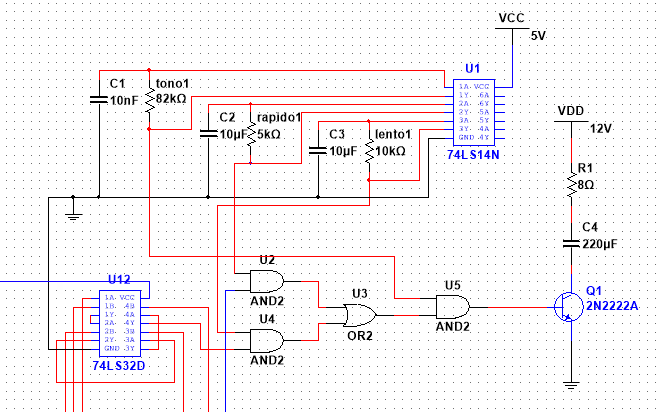
\includegraphics[width=0.7\textwidth]{circ audio.png}
		\caption{Diagrama del circuito de señalización auditiva.}
		\label{audio}
	\end{figure}

\subsection{Justificación de Diseño}
\begin{itemize}
	\item{Compuerta Schmitt Trigger 74LS14}
		Se selecciono un circuito integrado 74LS14 por la necesidad de generar señales cuadradas de un voltaje en corriente continua. Permite se manera sencilla implementar osciladores RC con bastante estabilidad evitando problemas de ruido y transiciones. Ademas, permite la generación de varios osciladores con un mismo circuito conectando una entrada y salida mediante una resistencia y un capacitor entre la entrada y tierra. Esto genera que conforme los valores elegidos de cada componente y según la carga o descarga del capacitor se genere de manera simple una señal cuadrada.
	\item{Compuertas AND/OR}
		Permiten procesar la lógica necesaria para que no haya bugs en el sistema. Permiten una selección de velocidad de pitidos y una mezcla de estos con la señal audible.
	\item{Transistor NPN}
		El transistor NPN fue seleccionado debido a que las compuertas lógicas no son capaces de suministrar la corriente necesaria para alimentar directamente el parlante. El transistor añade corriente y por ende potencia entre la lógica digital y logra que la carga de salida sea audible más fácilmente.
		Como beneficio adicional, esta configuración protege las compuertas lógicas contra sobrecorrientes y permite utilizar una fuente de alimentación de mayor voltaje para aumentar el volumen del sonido emitido.
	\item{Resistencia de Base}
		La resistencia conectada a la base del transistor limita la corriente de entrada, evitando daños tanto en la salida lógica como en el transistor. Este componente resulta fundamental para garantizar una operación segura del sistema.
	\item{Parlante}
		Se utilizó un parlante de baja impedancia como dispositivo de salida debido a su simplicidad y facilidad de integración. El uso de ondas cuadradas permite generar tonos audibles claramente distinguibles sin necesidad de circuitos de audio complejos.
\end{itemize}

\subsection{Gráficas}

\begin{figure}[H]
    \centering
    \begin{minipage}{0.45\textwidth}
        \centering
        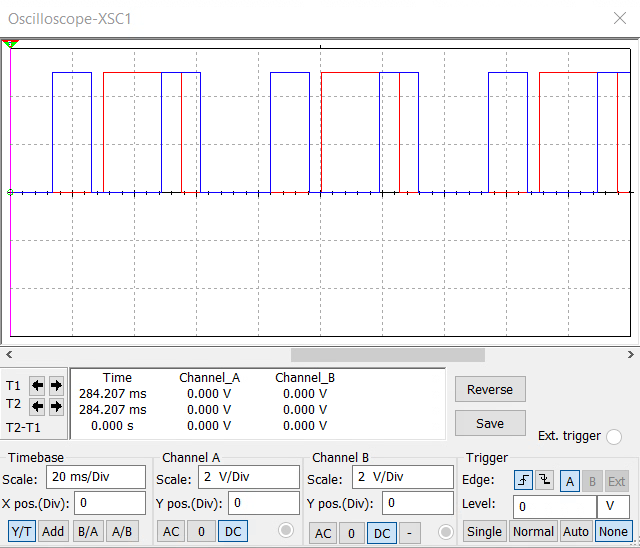
\includegraphics[width=0.9\textwidth]{osc velocidad.png}
		\caption{Señal de oscilación segun seleccion de velocidad.}
    \end{minipage}
    \hfill
    \begin{minipage}{0.45\textwidth}
        \centering
        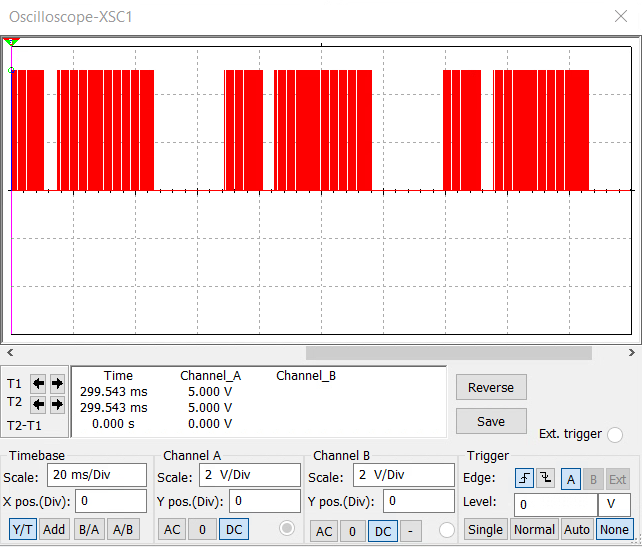
\includegraphics[width=0.9\textwidth]{salida lento.png}
		\caption{Ejemplo de tono de salida en modo lento.}
    \end{minipage}

\end{figure}

\end{document}
